\documentclass{beamer}
\usepackage{beamerthemesplit}

%\usepackage{pgfpages}
%\pgfpagesuselayout{resize to}[a4paper,landscape,border shrink=5mm]
%\pgfpagesuselayout{2 on 1}[a4paper,portrait,border shrink=5mm]
%\pgfpagesuselayout{8 on 1}[a4paper,portrait,border shrink=5mm]

\usepackage{ngerman}
\usepackage[applemac]{inputenc}
\usepackage{colortbl}
\usepackage{hyperref} 

\date{\today}
\author{markus.degen@fhnw.ch}
\institute{FHNW}
\logo{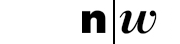
\includegraphics[height=0.4cm]{../fhnw.png}}
\title {Netzwerke und Datenkommunikation}

\newcommand{\orangecell}{{\cellcolor[rgb]{0.98,0.83,0}}}
\newcommand{\greencell}{{\cellcolor[rgb]{0.4,0.9,0.3}}}
\newcommand{\graycell}{{\cellcolor[gray]{0.8}}}
\newcommand{\olivecell}{{\cellcolor[rgb]{0.6,0.8,0.2}}}
\newcommand{\steelcell}{{\cellcolor[rgb]{0.7,0.8,0.9}}}
\newcommand{\linksymbol}{\tiny{$\hookrightarrow$}}
\newcommand{\myurl}[1]{{\color{violet}{\tiny{\url{#1}}}}}

\renewcommand{\figurename}{Fig}

\usetheme[secheader]{Boadilla}
%\setbeamercolor*{palette primary}{use=structure,fg=black,bg=green!5!white}
%\setbeamercolor*{palette secondary}{use=structure,fg=black,bg=green!15!white}
%\setbeamercolor*{palette tertiary}{use=structure,fg=black,bg=green!25!white}
%\setbeamercolor*{palette quaternary}{fg=white,fg=red}

\setbeamercolor*{palette primary}{use=structure,fg=black,bg=green!25!yellow!35!white!70}
\setbeamercolor*{palette secondary}{use=structure,fg=black,bg=green!35!yellow!45!white!70}
\setbeamercolor*{palette tertiary}{use=structure,fg=black,bg=green!45!yellow!65!white!70}
\setbeamercolor*{palette quaternary}{fg=white,fg=red}


\begin{document} % ===============================================================

\section{ND07: Transportschicht im Internet}
\subsection{\"Ubersicht}

\frame {
\frametitle{Unterrichtsbl�cke} %------------------------------------------
\small
\begin{tabular}{|p{0.02\textwidth}|p{0.7\textwidth}|p{0.18\textwidth}|}
\hline
{\cellcolor[gray]{0.8}} Bl & {\cellcolor[gray]{0.8}} Inhalt  & {\cellcolor[gray]{0.8}} Buch \\ \hline
01 &  Einleitung, \"Ubersicht, Grundbegriffe  & \tiny{}\\ \hline
02 & OSI-Modell: L1 und L2 & \tiny{} \\ \hline
03 & OSI-Modell: L2 und L3 &\tiny{}\\ \hline
04 & OSI-Modell: L3 bis L7 &\tiny{} \\ \hline
05 & IP (Adressierung) & \tiny{} \\ \hline
06 &  IP (ARP, ICMP) & \tiny{} \\ \hline
07 & Labor  & \tiny{} \\ \hline
\orangecell 08 & \orangecell TCP &  \orangecell \tiny{598-601} \\ \hline
09 & Internet & \tiny{} \\  \hline

10 & Anwendungsprotokolle: DNS & \tiny{} \\ \hline
11 & Anwendungsprotokolle: DHCP, Mail, rLogin & \tiny{} \\ \hline
12 & Labor & \tiny{} \\ \hline
13 & Anwendungsprotokolle: HTTP (+HTML) &  \tiny{} \\ \hline
14 & Labor &  \tiny{} \\ \hline
15 & WLAN und Netzsicherheit &  \tiny{} \\ \hline
\end{tabular}
}


\frame { %------------------------------------------
\frametitle{ND07: Transportschicht im Internet} 
\textbf{Lernziele}
\begin{itemize}
\item Sie k\"onnen erkl\"aren, was die Hauptaufgaben und -Eigenschaften 
	von TCP sind, wie ein TCP-Paket grob aufgebaut ist 
\item Sie k\"onnen mit einem entsprechenden Tool TCP-Pakete auf dem 
	Ethernet auffangen und deren Inhalt interpretieren.
\end{itemize}
\textbf{Themen}
\begin{itemize}
\item TCP
\item UDP
\item \textbf{Labor:} Lern\"ubung zu TCP. Mit Ethereal/Wireshark TCP-Pakete auf 
	dem Ethernet aufzeichen und interpretieren.
\end{itemize}
}

\subsection{TCP}
\frame { %------------------------------------------
\frametitle{TCP (Transport Control Protocol)}
\begin{itemize}
\item Bereitstellen eines \alert{zuverl\"assigen} End-to-End Bytestromes 
	(Virtueller Kanal)
	\begin{itemize}
		\item Reihenfolge (Auf IP-Ebene beliebig) wird durch Sequenznummern
			festgelegt
		\item Retransmit bei Timeout
		\item Verwerfen von doppelten Paketen
	\end{itemize}
\item Die Endpunkte einer TCP-Verbindung werden \alert{Port}s genannt 
	\item Repr\"asentiert durch eine 16-Bit Zahl 
	\item Programmiertechnisch werden die Endpunkte als \alert{Socket} 
		bezeichnet
\item Die Flusssteuerung geschieht mittels \alert{sliding windows}
\item [$\rightarrow$] TCP ist im \alert {RFC 793} beschrieben
\end{itemize}
} 

\frame { %------------------------------------------
\frametitle{TCP Paket-Header}
\framesubtitle{Quelle: RFC 793}
\begin{center}
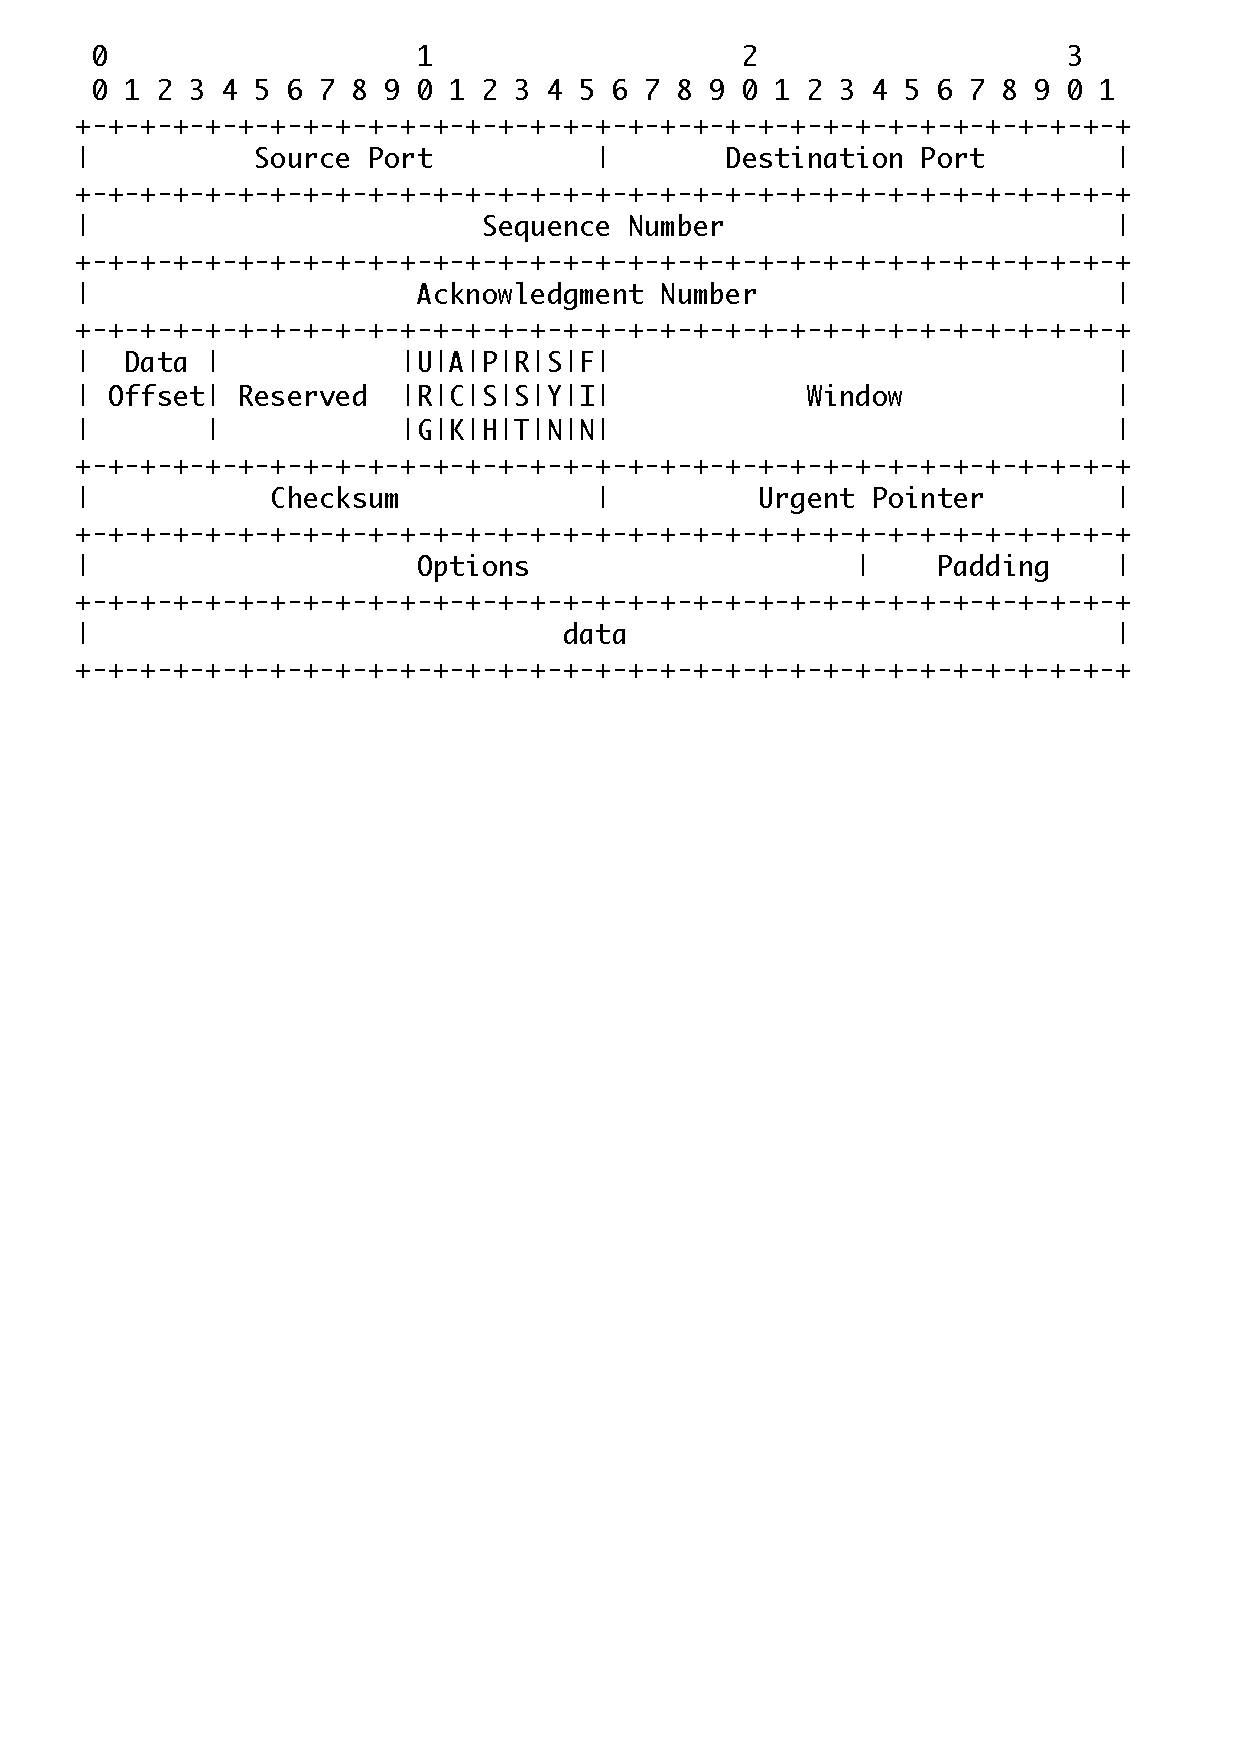
\includegraphics[width=0.9\textwidth]{tcpheader.pdf}
\end{center}
%\footnotetext[1]{\tiny{A. Tanenbaum, ''Computer Networks'', http://authors.phptr.com/tanenbaumcn4/}}
%\begin{figure}
%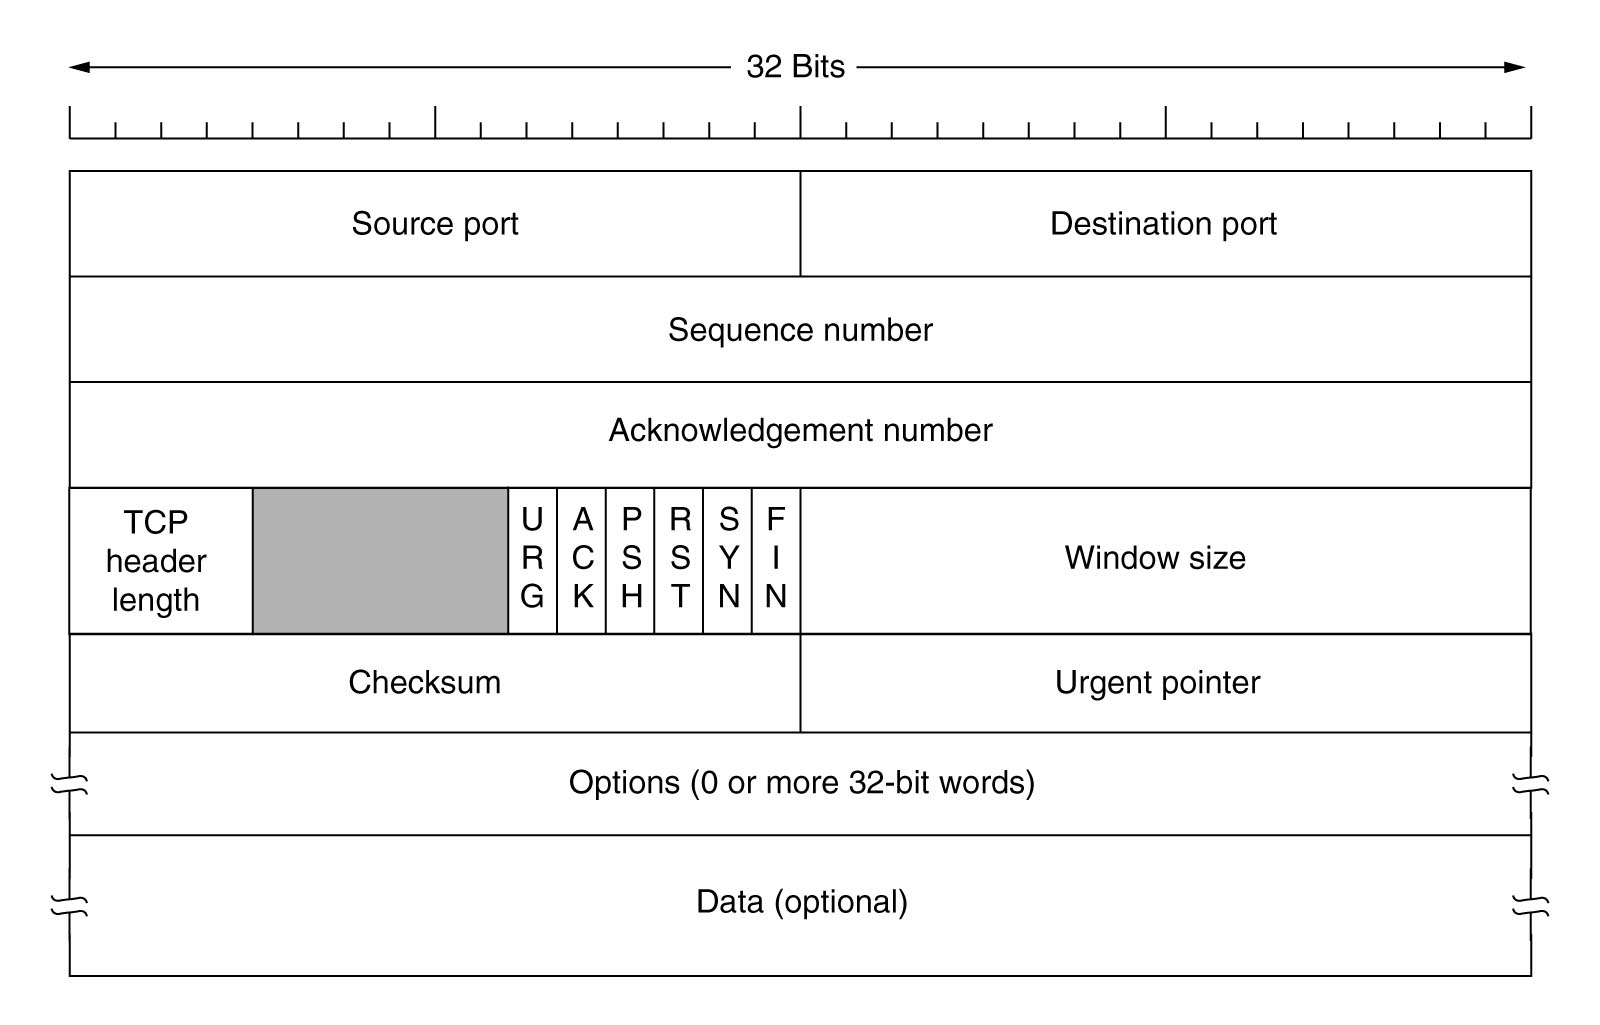
\includegraphics[width=0.75\textwidth]{6-29.jpg}
%\caption{ \tiny{6-29\footnotemark[1], TCP Header}}
%\end{figure}

} 

\frame { %------------------------------------------
\frametitle{TCP Headerfelder 1/2}
\begin{description}
\item [Source Port:] Portnummer der Quelle
\item [Destination Port:] Portnummer des Ziels
\item [Sequence Nbr:] Sequenznummer des ersten Bytes in diesem Segment 
	(Bei SYN=1: ISN (Initial Sequence Number)
\item [Ackn. Nbr:] Quittung, enth\"alt die Sequenznummer des n\"achsten
	erwarteten Bytes
\item [Data Offset:] Anzahl der 32-Bit Worte des Headers (Offset an dem die
	Daten beginnen)
\item [URG:] Wenn ''1'': Urgent-Pointer ist g\"ultig
\item [ACK:] Wenn ''1'': Acknowledgment Feld ist g\"ultig
\item [PSH:] Push-Funktion, wenn ''1'': Empf\"anger soll die Daten direkt weiterleiten,
	ohne darauf zu warten, bis der Puffer gef\"ullt ist

\end{description}
}


\frame { %------------------------------------------
\frametitle{TCP Headerfelder 2/2}
\begin{description}
\item [RST:] Wenn ''1'': Zur\"ucksetzen der Verbindung (Abweisen von unerw\"unschten
	Verbindungen, technische Probleme) 
\item [SYN:] Synchronisierung (Verbindungsaufbau)
\item [FIN:] Verbindungsabbau
\item [Window:] Gr\"osse des Schiebefensters, gibt an, wieviele Bytes gesendet
	werden k\"onnen
\item [Checksum:] Pr\"ufsumme
\item [Urgent Pointer:] Position der ''Urgent''-Daten im Datenstrom (selten benutzt)
\item [Options:] Weitere Optionen, z.B. Maximalgr\"osse des Datensegmentes
\item [Padding:] Fullbits umd auf eine 4-Wort-Grenze zu kommen
\item [(Data:] Nutzdaten, geh\"oren nicht mehr zum Header)
\end{description}
} 

\frame { %------------------------------------------
\frametitle{TCP  Verbindungsaufbau}
\footnotetext[1]{\tiny{A. Tanenbaum, ''Computer Networks'', http://authors.phptr.com/tanenbaumcn4/}}
\begin{figure}
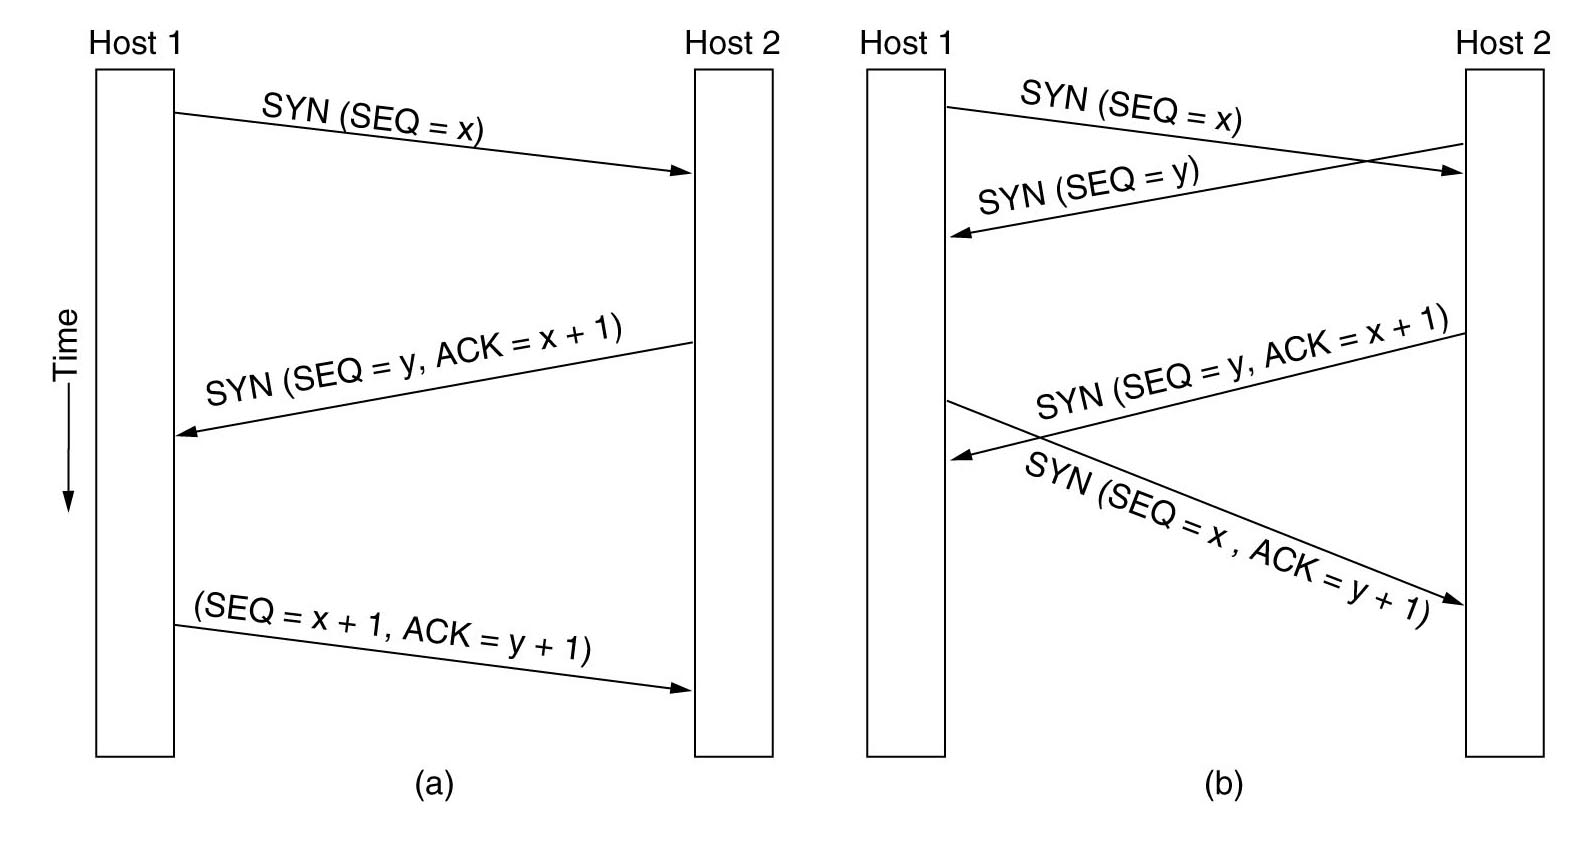
\includegraphics[width=0.95\textwidth]{6-31.jpg}
\caption{ \tiny{6-31\footnotemark[1], Verbindungsaufbau}}
\end{figure}
} 

\frame { %------------------------------------------
\frametitle{TCP  Verbindungsaufbau (wireshark)}
\begin{center}
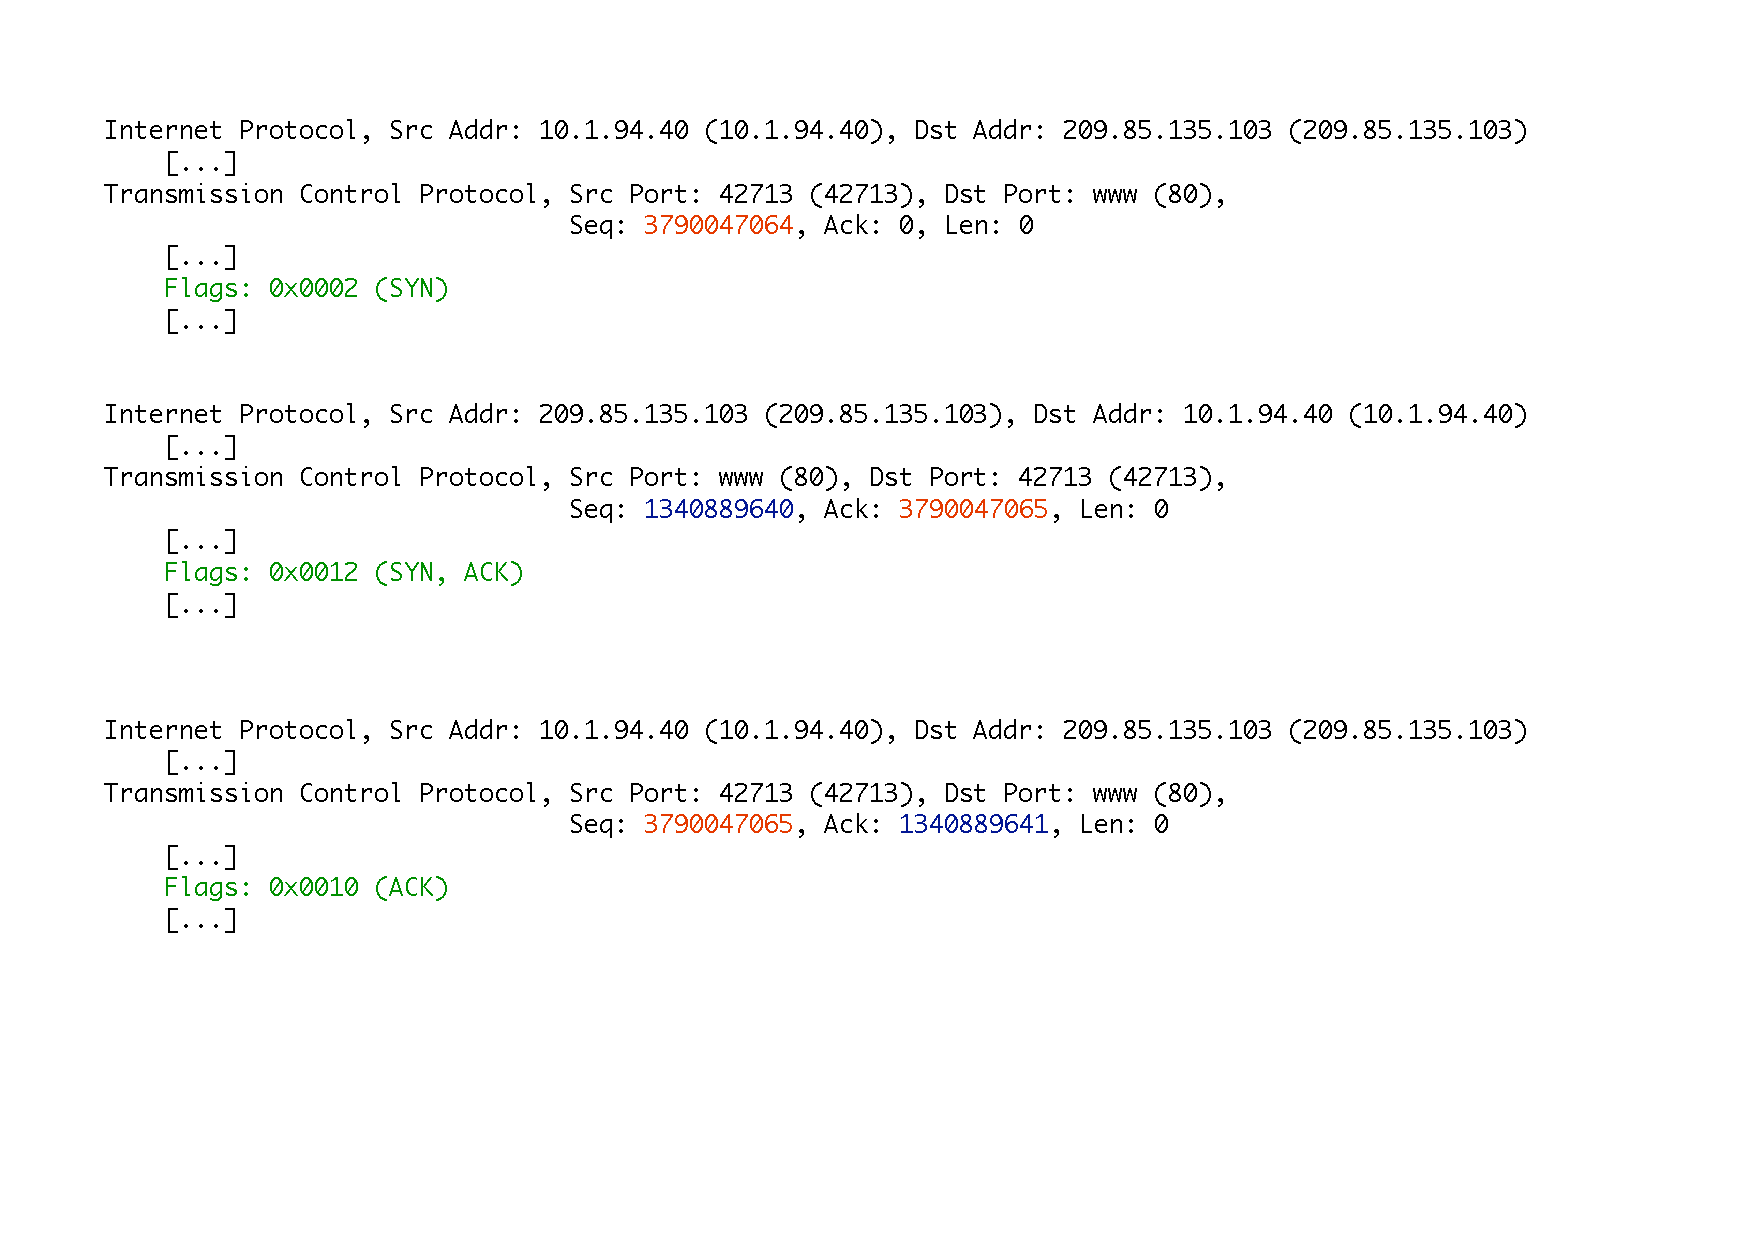
\includegraphics[width=\textwidth]{3wayhandshake.pdf}
\end{center}
}


\frame { %------------------------------------------
\frametitle{TCP  Verbindungsabbau}
\footnotetext[1]{\tiny{A. Tanenbaum, ''Computer Networks'', http://authors.phptr.com/tanenbaumcn4/}}
\begin{figure}
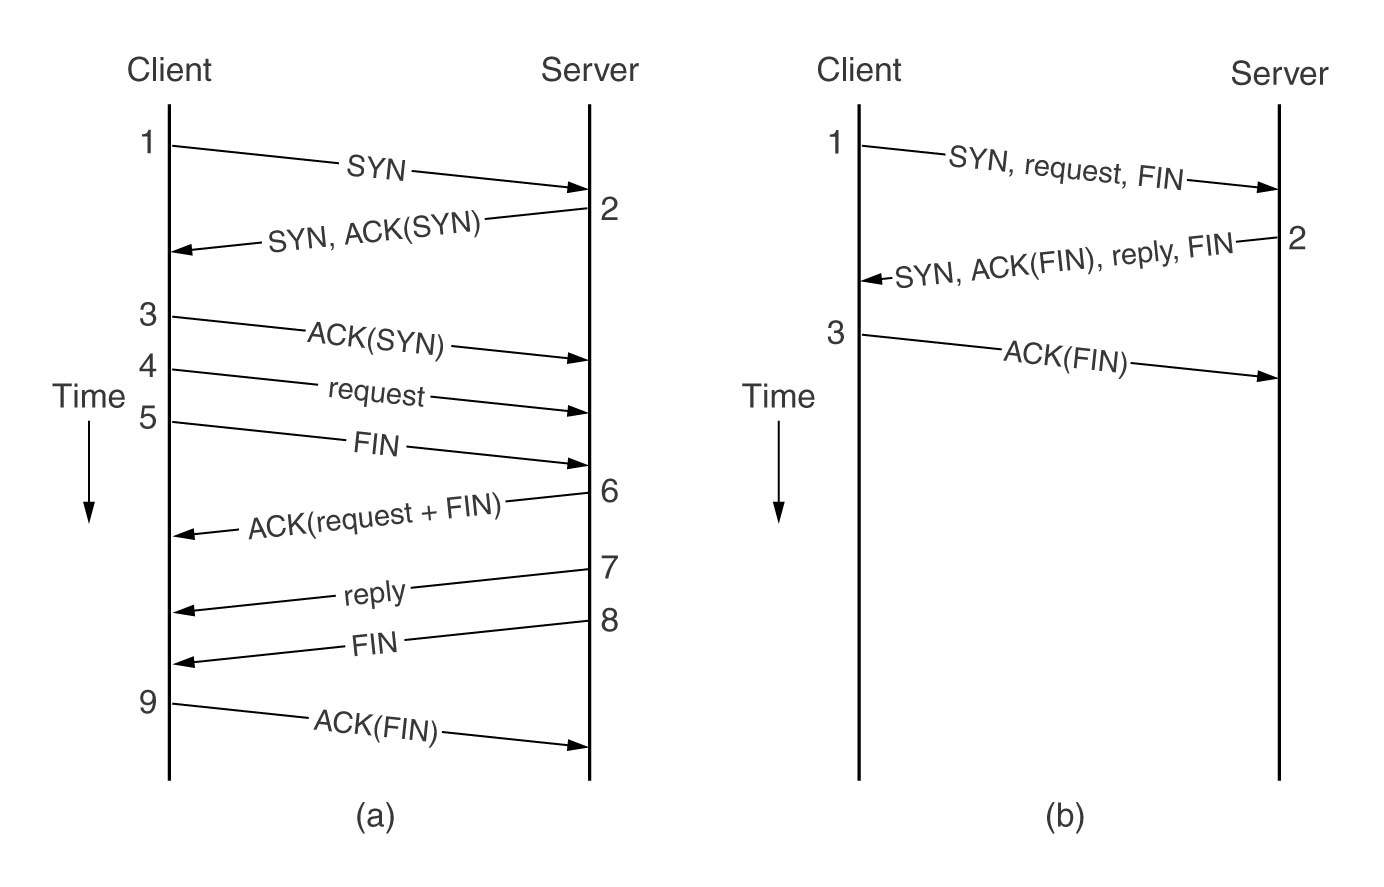
\includegraphics[width=0.8\textwidth]{6-40.jpg}
\caption{ \tiny{6-40\footnotemark[1], Verbindungsabbau}}
\end{figure}
}

\frame { %------------------------------------------
\frametitle{TCP: State-Event Diagramm}
\footnotetext[1]{\tiny{A. Tanenbaum, ''Computer Networks'', http://authors.phptr.com/tanenbaumcn4/}}
\begin{figure}
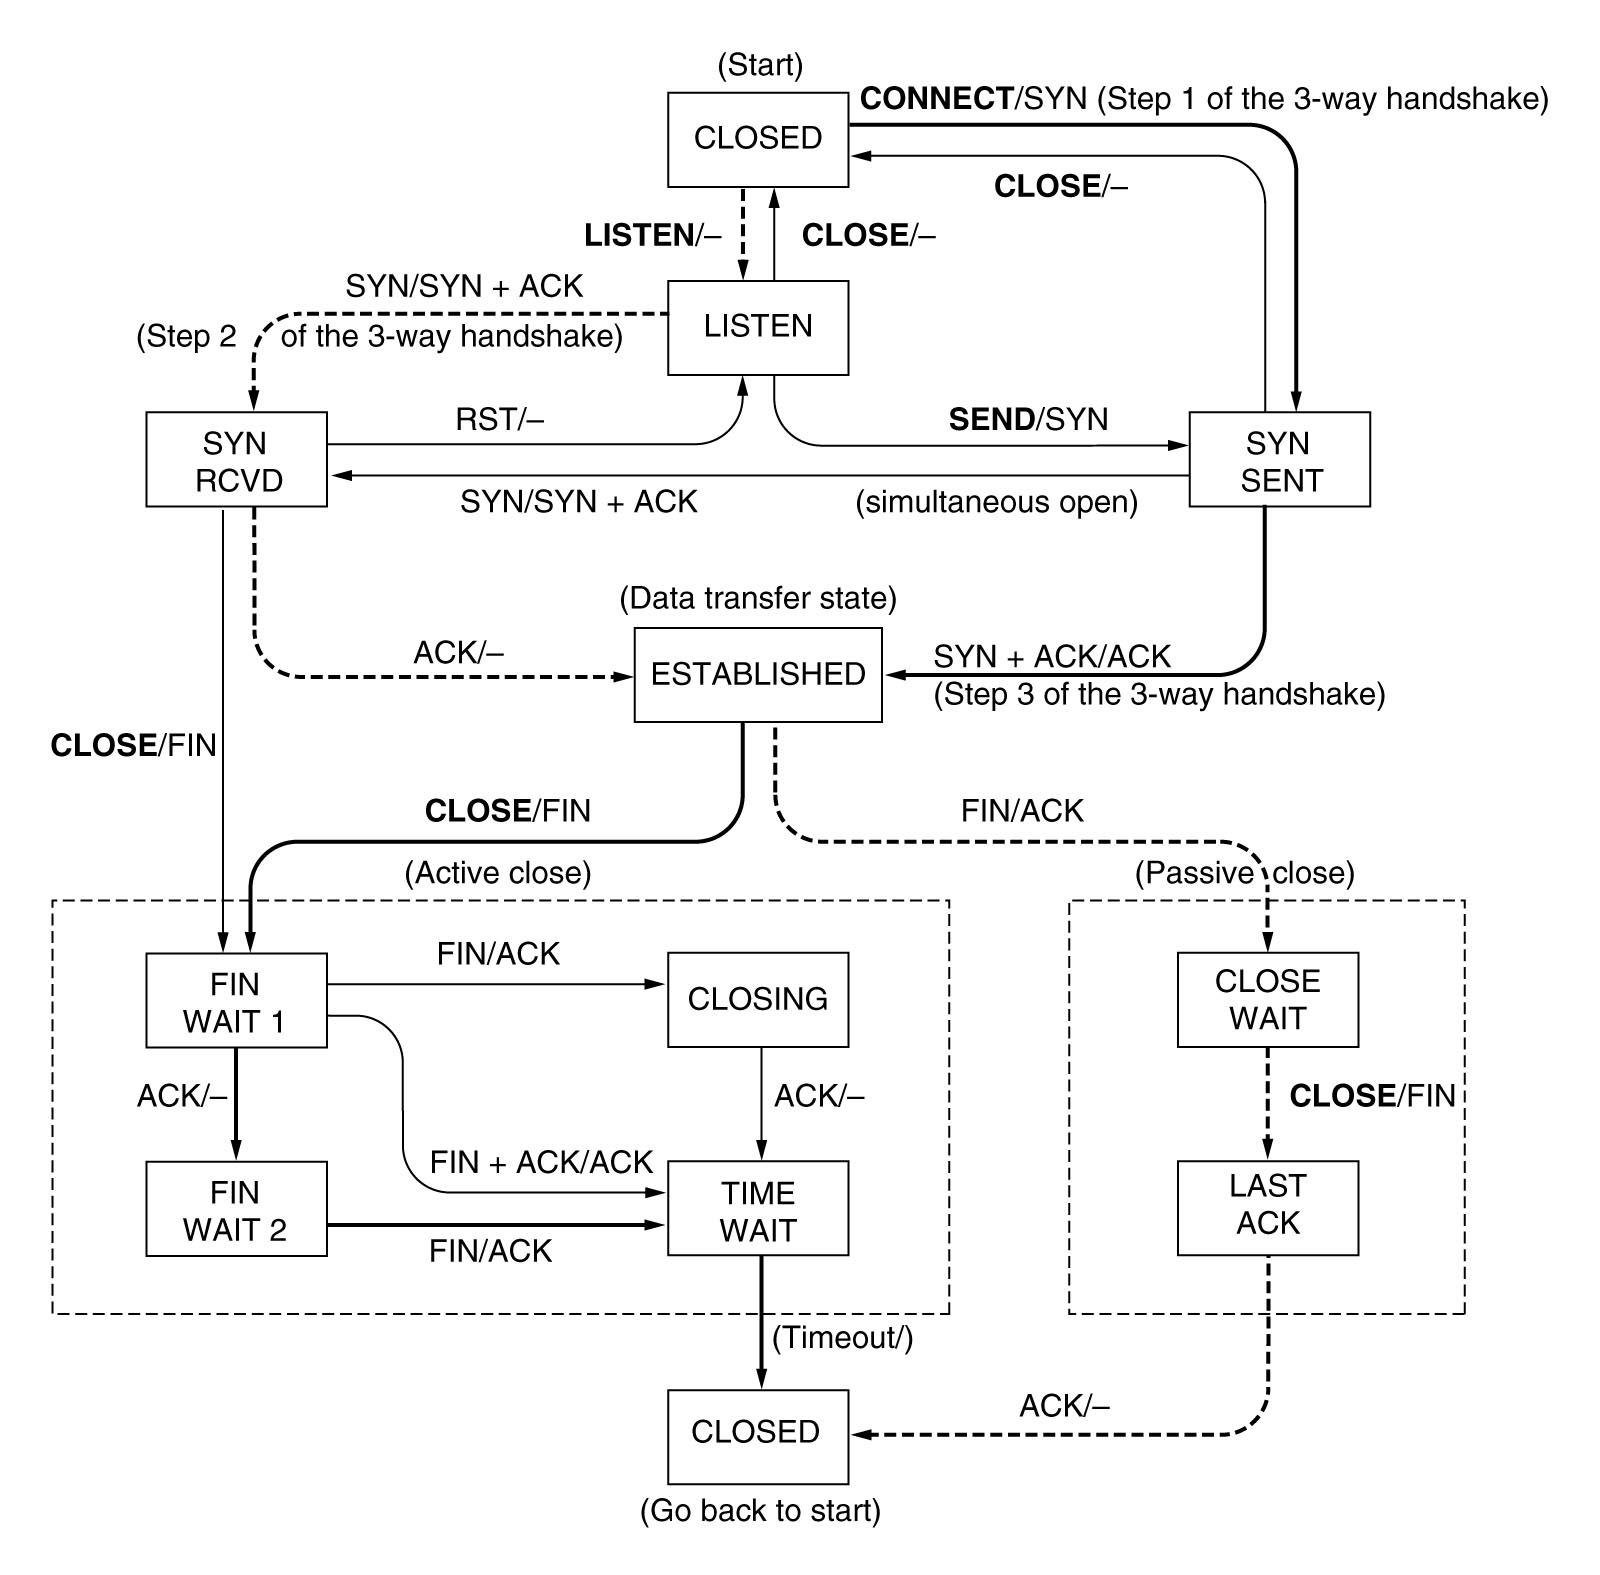
\includegraphics[width=0.5\textwidth]{6-33.jpg}
\caption{ \tiny{6-33\footnotemark[1], Verbindungsabbau}}
\end{figure}
}

\subsection{UDP}
\frame { %------------------------------------------
\frametitle{UDP: User Datagram Protocol}
\begin{itemize}
\item Verbindungsloses, unzuverl\"assiges Transportprotokoll
\begin{itemize}
\item Pakete k\"onnen verlorengehen, in der falschen Reihenfolge
	oder doppelt eintreffen
\end{itemize}
\item Einfacher als TCP, erfordert keinen Verbindungsauf 
	und -abbau
\item Unterst\"utzt keine Flusskontrolle
\item Geringere Netzwerk- und Ressourcenbelastung 
\item Das DNS (Domain Name System) benutzt z.B. UDP
\item [$\rightarrow$] UDP ist im \alert {RFC 768} beschrieben
\end{itemize}
}


\frame { %------------------------------------------
\frametitle{UDP Paket-Header}
\framesubtitle{Quelle: RFC 768}
Der UDP-Header ist sehr einfach und 8 Byte lang. Das Pr\"ufsummenfeld muss nicht
benutzt werden, dann kann es auf ''0'' gesetzt werden.
\begin{center}
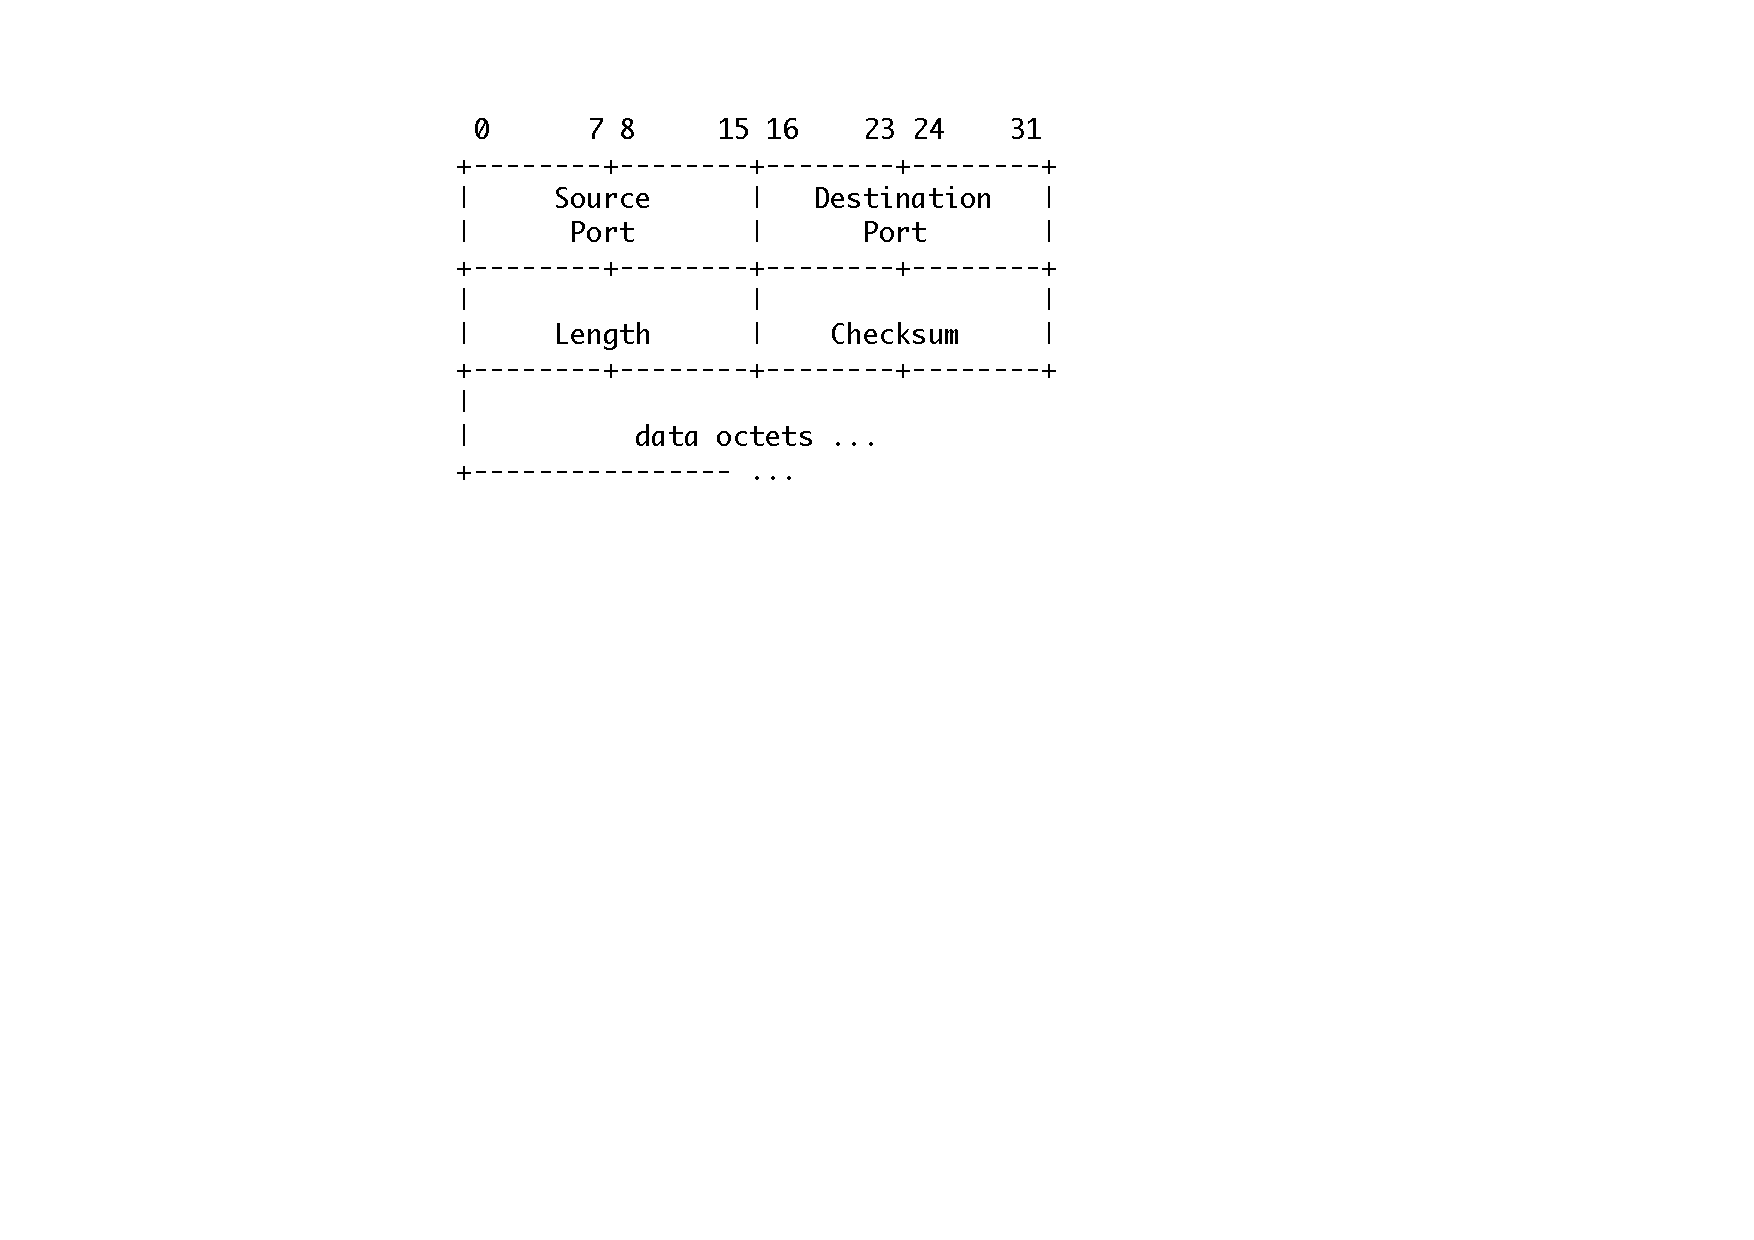
\includegraphics[width=0.7\textwidth]{udpheader.pdf}
\end{center}
}

\frame { %------------------------------------------
\frametitle{FTP (File Transfer Protocol)}
\begin{itemize}
\item FTP ist ein Anwendungsprotokoll zur Datei�bertragung in
	TCP/IP Netzen und ist im \alert {RFC 959} beschrieben
\item Dateien k�nnen sowohl vom Client auf den Server, wie auch
	vom Server auf den Client �bertragen werden.
\item Das FTP-Protokoll wird zwischen einem \alert{FTP-Server Prozess}
	und einem \alert{FTP-Client Prozess} eingesetzt, wobei der
	FTP-Client h�ufig ein User-Interface hat
\end{itemize}
\begin{center}
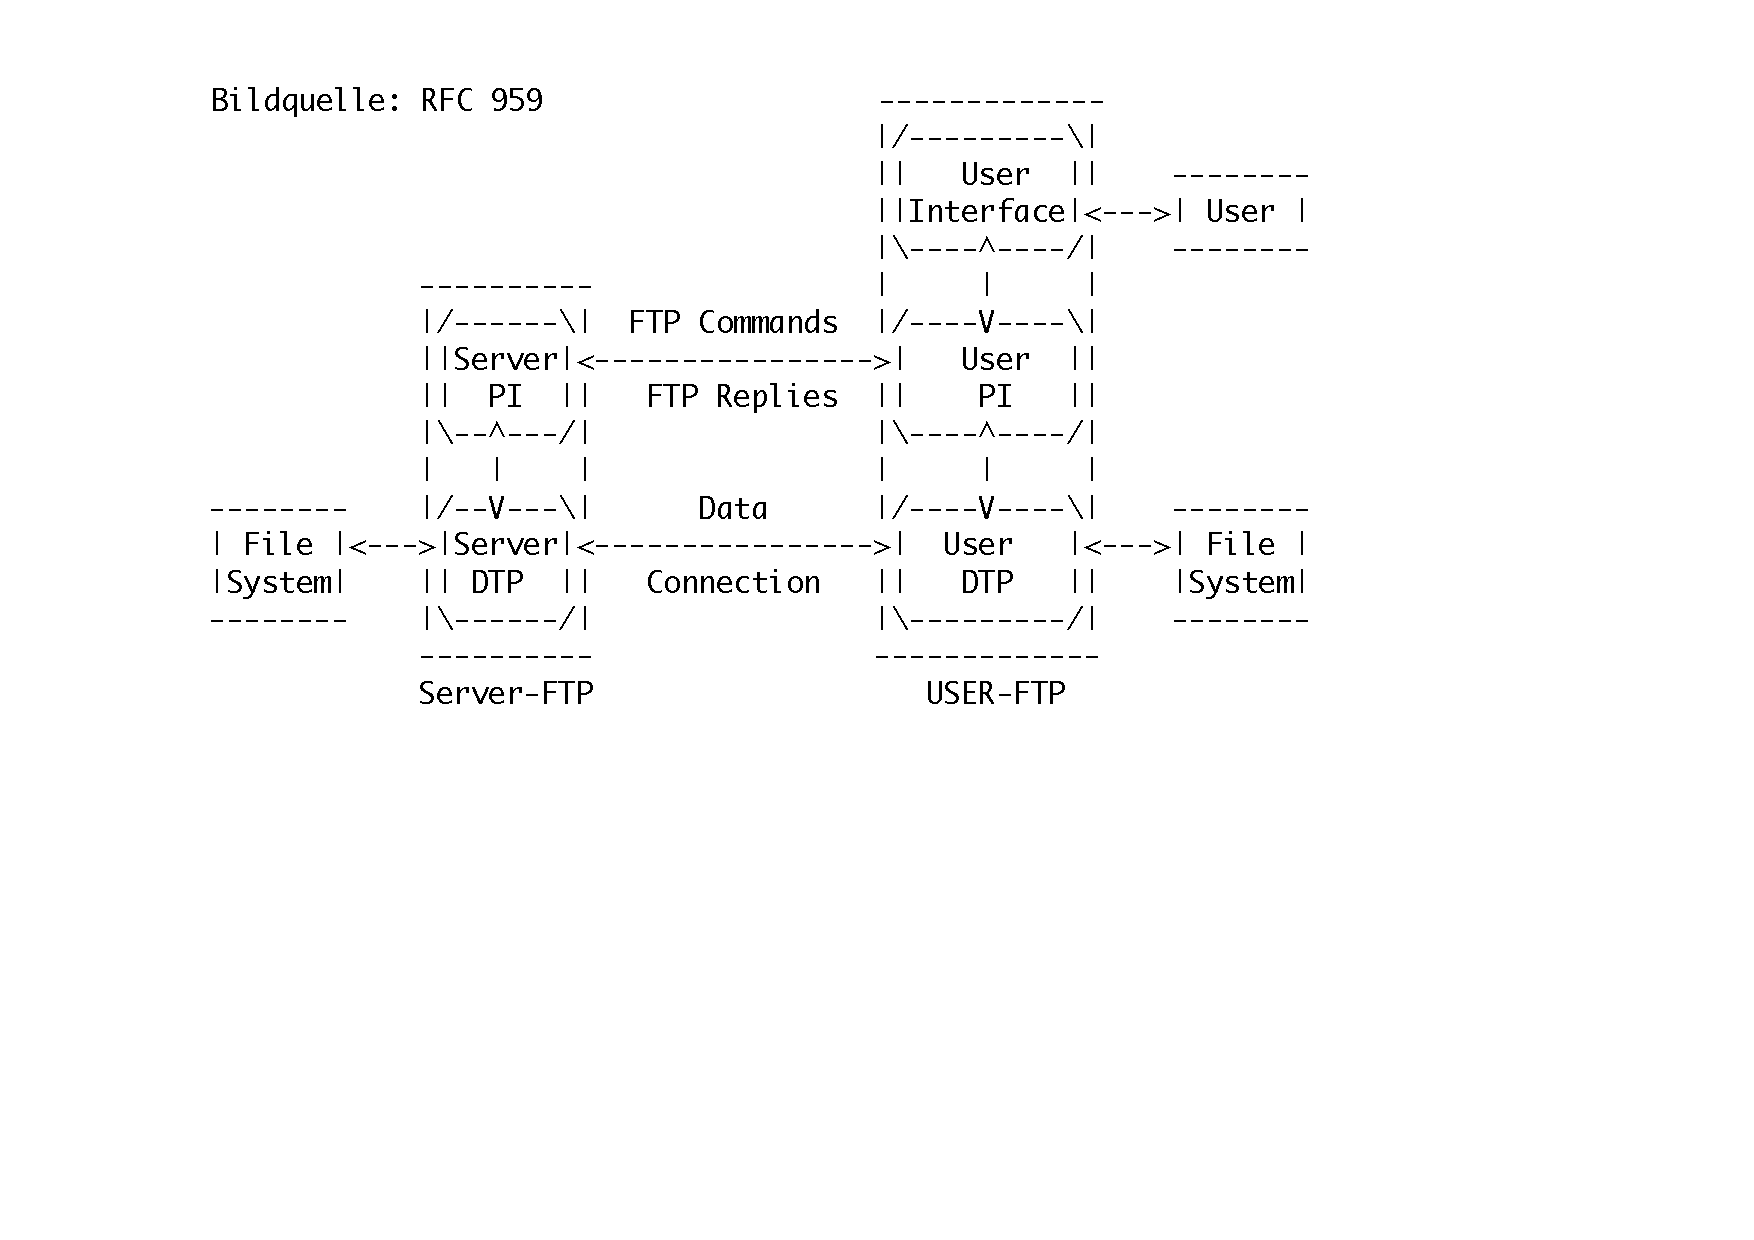
\includegraphics[width=0.62\textwidth]{ftpprinciple.pdf}
\end{center}
}

\frame { %------------------------------------------
\frametitle{FTP Session Example}
\begin{center}
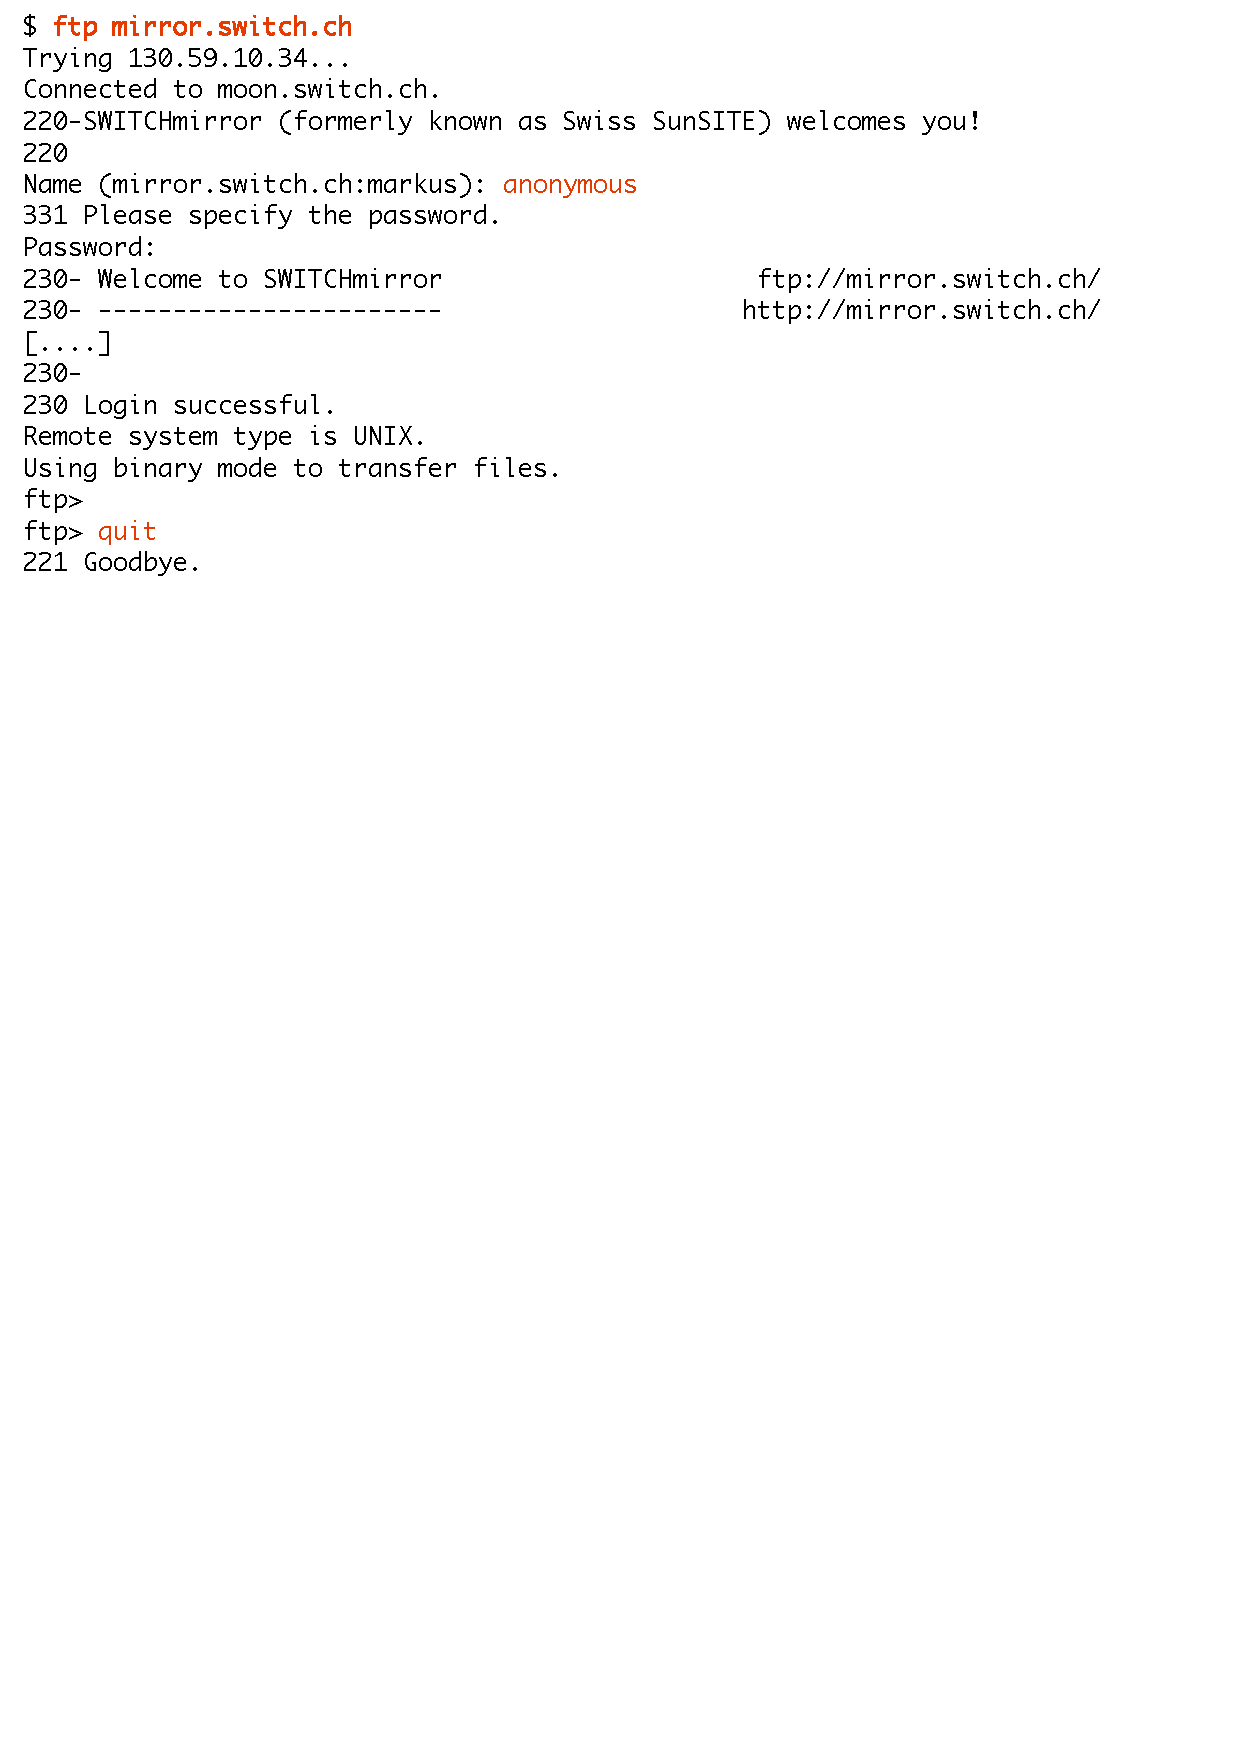
\includegraphics[width=\textwidth]{ftpexample.pdf}
\end{center}
}


%\footnotetext[1]{\tiny{A. Tanenbaum, ''Computer Networks'', http://authors.phptr.com/tanenbaumcn4/}}
%\begin{figure}
%\includegraphics[width=0.95\textwidth]{5-53.jpg}
%\caption{ \tiny{5-53\footnotemark[1], IPv4 Header}}
%\end{figure}
%}

%\begin{center}
%\includegraphics[width=0.7\textwidth]{osilayer1.pdf}
%\end{center}

\subsection{Abschluss}
\frame { %------------------------------------------
\frametitle{Abschluss} 
\footnotesize
\textbf{Behandelte Themen:}
\begin{itemize}
\item Transportschicht: TCP und UDP
\item FTP als Beispiel f\"ur ein Anwendungsprotokoll
\end{itemize}
\textbf{M\"ogliche Pr\"ufungsfragen}
\begin{itemize}
\item Was unterscheidet die Adressierung auf Layer TCP von der Adressierung auf 
	Layer IP?
\item Welcher Unterschied besteht zwischen TCP und UDP, welches sind die Einsatzgebiete?
\end{itemize}
\textbf{Labor/Selbststudium}
\begin{itemize}
\item Lesen sie das RFC 793 und beantworten Sie dazu die Fragen auf der 
	Folgeseite
\item Labor\"ubung
\end{itemize}
}

\frame{
\frametitle{Fragen zum RFC 793}
\scriptsize
Suchen Sie die Antworten zu den folgenden Fragen im RFC 793. Es ist
nicht die Intention, dass Sie das komplette RFC lesen, vielmehr sollen
sie das RFC �berfliegen und dabei die Struktur und die Art der 
beschriebenen Information erfassen. Vergleichen und diskutieren Sie
die gefundenen Antworten mit einer Kollegin/einem Kollegen.
\begin{enumerate}
\scriptsize
\item Welche Informationen werden im Kontext von TCP unter einer ''connection'' zusammengefasst?
\item TCP bietet eine zuverl�ssige (reliable) Kommunikationsschicht,
	dies wird durch die Verwendung von ....... und Best�tigungen 
	(acknowledgments) erreicht. Garantiert TCP, dass die Daten beim
	\emph{Enduser} fehlerfrei ankommen? Wieso bzw. Wieso nicht?
\item Das TCP-Headerfield bietet Platz f�r zus�tzliche Optionen, 
	welche Optionen sind im RFC definiert?
\item Das RFC schl�gt die Wahl der ISN aufgrund einer internen
	Uhr vor. Wie lange dauert es bei der vorgeschlagenen Zeiteinheit,
	bis die selbe ISN wieder verwendet wird?
\item Wieso ist das aushandeln der ISN beim ''three way handshaking''
	�berhaupt notwendig?
\item Was tut ein Empf�nger, der im ''Listen'' State ist und ein 
	''RST'' kriegt?
\item Das RFC schl�gt ein Set von ''User Commands' vor, welche sind 
	dies?
\item Wenn der Status einer Verbindung ''LISTEN'' ist und ein
	''ACK'' empfangen wird, was wird die Reaktion sein?	
\item Welche Timeouts werden im RFC beschrieben? 
\item Was wird mit TCB bezeichnet? Kennen Sie eine �hnliche 
	Struktur aus dem Gebiet der Betriebssysteme?
\end{enumerate}
}

\frame{
\frametitle{Labor\"ubung zu TCP}
\footnotesize
\textbf{Vorbemerkung:} Die im folgenden vorgeschlagene \"Ubung ist als Leitfaden
f\"ur eigene Experimente gedacht. Geben Sie sich nicht damit zufrieden, die angegebenen
Kommandos einfach nur einzugeben; Beobachten Sie die Systemreaktion und reflektieren
sie die Ergebnisse.
\begin{itemize}
\footnotesize
\item Starten Sie Ihr System mit Knoppix, werden Sie Superuser und verifizieren Sie die
	Netzwerkkonnektivit\"at mit \texttt{ping}
\item Zeichnen Sie nun eine ganze FTP-Session mit ethereal/wireshark 
	auf, stellen 
	Sie dabei die Filterung vern\"unftig ein.
\item Analysieren Sie nun die Pakete, beachten Sie insbesondere die folgenden Punkte:
  \begin{itemize}
  \footnotesize
  \item 3-Way Handshake und initiale Sequenznummern
  \item Ihr eingegebenes Passwort
  \item Die seq und ack Felder (Sie k\"onnen die Nummerierung der von ''relativ'' auf
  	''absolut'' umstellen: Menue ''Edit''$\rightarrow$''Preferences''$\rightarrow$''Protocols''
	$\rightarrow$''TCP'' (Deselect Checkbox))
  \item Den Verbindungsabbau
  \item Die Pakete auf den verschiedenen Protokollschichten (FTP/TCP/IP/Ethernet), 
  	insbesondere auf die Adressierung.
  \end{itemize}
\end{itemize}
}




\end{document} 